\documentclass[11pt,a4paper]{article}
\usepackage[margin=2.2cm]{geometry}
\usepackage{amsmath,amssymb,bm}
\usepackage{graphicx,float,booktabs,caption,subcaption}
\usepackage{xcolor}
\usepackage{listings}
\usepackage{tikz}
\usetikzlibrary{shapes.geometric,arrows.meta,positioning,calc}
\usepackage[colorlinks=true,linkcolor=blue!50!black,urlcolor=blue!50!black,citecolor=blue!50!black]{hyperref}
\usepackage{fancyhdr}
\pagestyle{fancy}\fancyhf{}\lhead{\small Karthick J (OE23S018), IIT Madras}\rhead{\small\leftmark}\cfoot{\thepage}
\definecolor{codebg}{rgb}{0.97,0.97,0.97}
\lstset{basicstyle=\ttfamily\scriptsize,backgroundcolor=\color{codebg},frame=single,breaklines=true,
 keywordstyle=\color{blue!60!black}\bfseries,commentstyle=\color{green!40!black},stringstyle=\color{red!50!black},
 numbers=left,numberstyle=\tiny\color{gray},showstringspaces=false,tabsize=4,columns=fullflexible,
 literate={²}{{$^2$}}1 {³}{{$^3$}}1 {°}{{$^\circ$}}1 {Δ}{{$\Delta$}}1 {ρ}{{$\rho$}}1 {μ}{{$\mu$}}1 {ω}{{$\omega$}}1 {ψ}{{$\psi$}}1 {α}{{$\alpha$}}1 {ν}{{$\nu$}}1 {τ}{{$\tau$}}1 {–}{{-}}1 {—}{{-}}1 {’}{{'}}1 {“}{{"}}1 {”}{{"}}1 {→}{{$\to$}}1 {≤}{{$\le$}}1 {≥}{{$\ge$}}1 {×}{{$\times$}}1 {±}{{$\pm$}}1 {·}{{$\cdot$}}1 {∂}{{$\partial$}}1 {∇}{{$\nabla$}}1 {γ}{{$\gamma$}}1 {ε}{{$\varepsilon$}}1 {μ}{{$\mu$}}1 {├}{{+}}1 {─}{{-}}1 {│}{{|}}1 {▶}{{>}}1 {▼}{{v}}1 {┌}{{+}}1 {┐}{{+}}1 {└}{{+}}1 {┘}{{+}}1 {┬}{{+}}1 {┴}{{+}}1}
\tikzset{
 startstop/.style={rectangle,rounded corners=6pt,minimum width=3.2cm,minimum height=0.8cm,text centered,draw=black,fill=red!12,font=\small},
 process/.style={rectangle,minimum width=4.6cm,minimum height=0.8cm,text centered,text width=5.6cm,draw=black,fill=blue!8,font=\small},
 decision/.style={diamond,aspect=2.6,text centered,text width=3.2cm,draw=black,fill=green!12,font=\small,inner sep=1pt},
 io/.style={trapezium,trapezium left angle=72,trapezium right angle=108,minimum width=3.6cm,minimum height=0.8cm,text centered,text width=4.6cm,draw=black,fill=orange!15,font=\small},
 arrow/.style={thick,-{Stealth[length=2.5mm]}}}
\setlength{\parskip}{4pt}\setlength{\parindent}{0pt}

\title{\textbf{One-Dimensional Advection--Diffusion of a Dye Release}\\[2pt]\large Explicit Upwind/Central Finite-Difference Solution in C, with Modified-Equation Analysis\\[2pt]\normalsize Course Project 3 -- OE5450 Numerical Techniques in Ocean Hydrodynamics (Tutorial 5, Jan--May 2025)}
\author{Karthick J (OE23S018)\\Department of Ocean Engineering, IIT Madras\\Faculty: Prof.\ K.\ Murali}
\date{Revised report, October 2026}
\begin{document}\maketitle
\begin{abstract}
The transport of an instantaneous dye release ($C_0=10$~kg\,m$^{-3}$ at one node) in a uniform stream is computed for $u=0$, 1, 1.5 and 2~m\,s$^{-1}$ with $D=0.5$~m$^2$s$^{-1}$, using forward-Euler time integration, first-order upwind advection and central diffusion. The C code printed in the original report did not compile (a missing semicolon and an illegal initialiser on variable-length arrays); after these two corrections it reproduces the original results file exactly. Comparison with the exact Gaussian (Green's function) solution shows that the computed plume is systematically wider and lower than the physical one when $u>0$. A modified-equation analysis attributes this to an artificial diffusion $D_{num}=\tfrac12u\Delta x(1-\mathrm{CFL})$, which equals 19\% and 36\% of the physical diffusivity at $u=1$ and 2~m\,s$^{-1}$. Moment analysis of the computed fields confirms the prediction: the effective diffusivities obtained from $d\sigma^2/dt$ are 0.593, 0.639 and 0.676~m$^2$s$^{-1}$ against the predicted 0.595, 0.639 and 0.680~m$^2$s$^{-1}$, and the plume centroid travels at $u$ to within 0.1\%.
\end{abstract}
\tableofcontents\newpage

\section{Problem definition}
A dye is injected into a uniform one-dimensional flow. Its concentration $C(x,t)$ obeys
\begin{equation}
\frac{\partial C}{\partial t}+u\frac{\partial C}{\partial x}=D\frac{\partial^2 C}{\partial x^2},\qquad -10\le x\le10~\mathrm{m},\quad t>0, \label{eq:ad}
\end{equation}
with $D=0.5$~m$^2$s$^{-1}$ and $u\in\{0,\,1.0,\,1.5,\,2.0\}$~m\,s$^{-1}$ ($u=1.5$ was the last case run in the original work). The dye is released once, at $t=0$, as a single-node spike $C(0,0)=C_0=10$~kg\,m$^{-3}$, i.e.\ a mass per unit area $M=C_0\Delta x=2$~kg\,m$^{-2}$. The ends are held at $C=0$. (The code's title mentions a ``continuous source'', but the update never re-injects dye; the problem actually solved is an instantaneous release, which is also what the original plots show.)

\subsection{Exact solution}
For an infinite domain the solution is the advected heat kernel
\begin{equation}
C(x,t)=\frac{M}{\sqrt{4\pi Dt}}\exp\!\left[-\frac{(x-ut)^2}{4Dt}\right], \label{eq:exact}
\end{equation}
whose moments are $\int C\,dx=M$, $\bar x=ut$ and $\sigma^2=2Dt$. It is valid for the finite domain as long as the plume ($\bar x\pm3\sigma$) has not reached $x=\pm10$~m.

\subsection{Non-dimensional parameters}
\begin{table}[H]\centering\small
\begin{tabular}{lcccc}\toprule
$u$ (m/s) & 0 & 1.0 & 1.5 & 2.0\\\midrule
$\mathrm{CFL}=u\Delta t/\Delta x$ & 0 & 0.05 & 0.075 & 0.10\\
$d=D\Delta t/\Delta x^2$ & 0.125 & 0.125 & 0.125 & 0.125\\
cell P\'eclet $\mathrm{Pe}_\Delta=u\Delta x/D$ & 0 & 0.4 & 0.6 & 0.8\\
domain P\'eclet $uL/D$ & 0 & 40 & 60 & 80\\
$D_{num}=\tfrac12u\Delta x(1-\mathrm{CFL})$ (m$^2$/s) & 0 & 0.095 & 0.139 & 0.180\\
$D_{num}/D$ & 0 & 19\% & 28\% & 36\%\\\bottomrule
\end{tabular}\caption{Grid ($\Delta x=0.2$~m, 101 nodes; $\Delta t=0.01$~s) and flow parameters.}\end{table}

\section{Numerical method}
\subsection{Discretisation}
\begin{equation}
C_i^{n+1}=C_i^n-\mathrm{CFL}\,(C_i^n-C_{i-1}^n)+d\,(C_{i+1}^n-2C_i^n+C_{i-1}^n),\qquad i=1,\dots,N_x-2, \label{eq:scheme}
\end{equation}
i.e.\ forward-time, backward (upwind for $u\ge0$) space for advection and central space for diffusion, with $C_0^{n+1}=C_{N_x-1}^{n+1}=0$.

\subsection{Stability}
With $\theta=k\Delta x$ the von Neumann amplification factor of \eqref{eq:scheme} is
\begin{equation}
G(\theta)=1-(\mathrm{CFL}+2d)(1-\cos\theta)-\mathrm{i}\,\mathrm{CFL}\sin\theta ,
\end{equation}
and $|G|\le1$ for all $\theta$ requires $\mathrm{CFL}+2d\le1$ (together with $\mathrm{CFL}^2\le\mathrm{CFL}+2d$). Here $\mathrm{CFL}+2d\le0.35$, so every case is stable; and since all coefficients of \eqref{eq:scheme} are non-negative the scheme is also monotone (no new extrema, $C\ge0$).

\subsection{Modified equation and numerical diffusion}
Taylor-expanding \eqref{eq:scheme} about $(x_i,t^n)$ and eliminating $C_{tt}$ with the PDE ($C_{tt}=u^2C_{xx}+\dots$) gives the equation that the scheme actually solves:
\begin{equation}
C_t+uC_x=\Big[D+\underbrace{\tfrac12u\Delta x\,(1-\mathrm{CFL})}_{D_{num}}\Big]C_{xx}+\mathcal{O}(\Delta x^2,\Delta t^2,\Delta x\Delta t).
\end{equation}
The leading error is therefore an \emph{extra diffusion}, from the first-order upwind difference ($+\tfrac12u\Delta x$) partly cancelled by the forward-Euler time error ($-\tfrac12u^2\Delta t$). The computed plume should behave like \eqref{eq:exact} with $D$ replaced by $D_{eff}=D+D_{num}$. This prediction is tested in Section~\ref{sec:moments}.

\subsection{Algorithm}
\begin{figure}[H]\centering
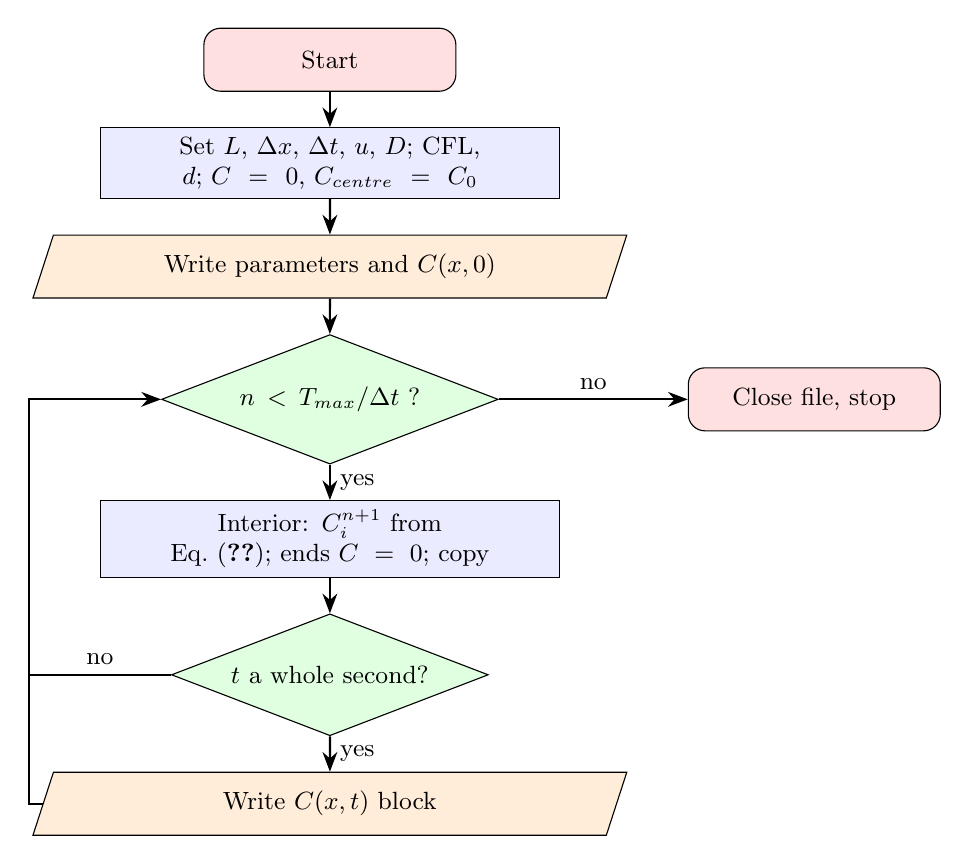
\begin{tikzpicture}[node distance=0.45cm]
\node(s)[startstop]{Start};
\node(i)[process,below=of s]{Set $L$, $\Delta x$, $\Delta t$, $u$, $D$; CFL, $d$; $C=0$, $C_{centre}=C_0$};
\node(w0)[io,below=of i]{Write parameters and $C(x,0)$};
\node(l)[decision,below=of w0]{$n<T_{max}/\Delta t$ ?};
\node(u)[process,below=of l]{Interior: $C^{n+1}_i$ from Eq.~(\ref{eq:scheme}); ends $C=0$; copy};
\node(q)[decision,below=of u]{$t$ a whole second?};
\node(w)[io,below=of q]{Write $C(x,t)$ block};
\node(e)[startstop,right=2.4cm of l]{Close file, stop};
\draw[arrow](s)--(i);\draw[arrow](i)--(w0);\draw[arrow](w0)--(l);\draw[arrow](l)--node[right,font=\small]{yes}(u);\draw[arrow](u)--(q);
\draw[arrow](q)--node[right,font=\small]{yes}(w);
\coordinate(LL) at ($(u.west)+(-0.9,0)$);
\draw[arrow](w.west)-|(LL)|-(l.west);
\draw[thick](q.west)--node[above,font=\small]{no}(q.west -| LL);
\draw[arrow](l)--node[above,font=\small]{no}(e);
\end{tikzpicture}
\caption{Flowchart of \texttt{code/advection\_diffusion.c}.}\end{figure}

\section{Code review and corrections}
The source code was taken from the original report (no separate source file was kept). Two compile errors were found and corrected; the method, parameters and output format are unchanged.
\begin{table}[H]\centering\small
\begin{tabular}{p{4.2cm}p{6.2cm}p{4.6cm}}\toprule
Location & Problem & Correction\\\midrule
\texttt{current\_time = (n + 1) * DT} & Missing semicolon: compile error. & Semicolon added.\\
\texttt{double C\_old[NX] = \{0.0\};} & \texttt{NX} is \texttt{(int)(L/DX)+1}, which is not an integer constant expression, so the arrays are variable-length arrays, which C does not allow to be initialised (compile error). & Declared without initialiser and zeroed in a loop.\\\bottomrule
\end{tabular}\caption{Corrections.}\end{table}
Points checked and left unchanged:
\begin{itemize}
\item The save test \texttt{fmod(current\_time,1.0) <= DT/2} was verified to catch all 100 whole-second instants, because the time is formed as $(n+1)\Delta t$ rather than accumulated. An integer step test would be more robust if $\Delta t$ were changed.
\item In the original gnuplot script, block \texttt{index 0} is the initial condition but is labelled ``Time = 1 s'', so every curve in the original figures carries a label one second too late. The new plots are labelled from the time stored in each block.
\end{itemize}
With the two corrections the program reproduces the original \texttt{results.txt} ($u=1.5$~m\,s$^{-1}$) exactly (maximum difference 0, Fig.~\ref{fig:orig}), so the run that produced the original figures used a correct copy of the code and the errors were introduced only in the printed listing.

\section{Results}
\subsection{Concentration profiles}
\begin{figure}[H]\centering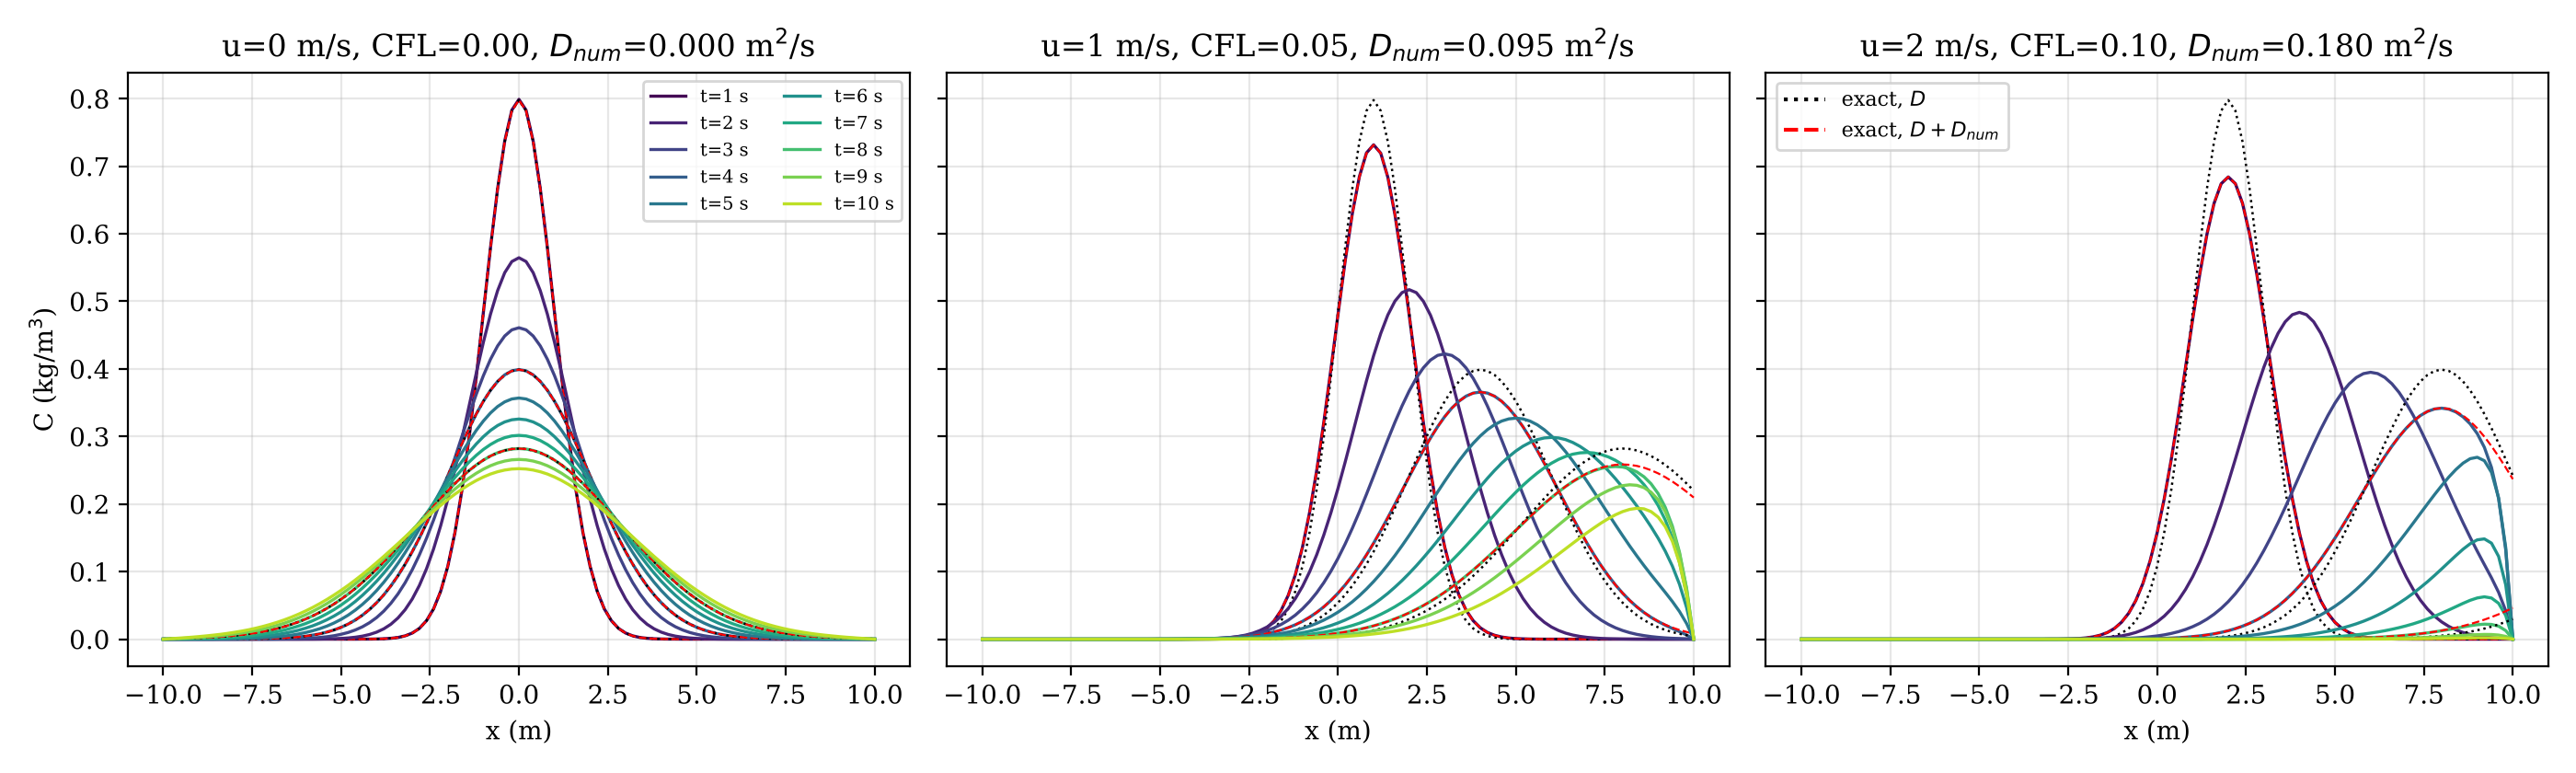
\includegraphics[width=\textwidth]{../results/fig1_profiles_vs_exact.png}
\caption{Computed profiles at $t=1,\dots,10$~s (solid) and the exact solution with the physical diffusivity $D$ (black dotted) and with $D_{eff}=D+D_{num}$ (red dashed) at $t=1,4,8$~s.}\end{figure}
For $u=0$ the computed Gaussian coincides with the exact solution (L$_2$ error $5\times10^{-5}$ at $t=4$~s; peak 0.3991 vs.\ 0.3989). For $u>0$ the computed plume is lower and wider than the physical solution but matches the exact solution evaluated with $D_{eff}$: at $t=4$~s the peak is 0.3657 for $u=1$ against 0.3989 with $D$ and 0.3657 with $D_{eff}$. At $u=2$ the plume reaches the outflow boundary after $\approx4$~s; the Dirichlet condition $C=0$ then acts as a perfect sink and produces the sharp drop at $x=10$~m. A zero-gradient outflow condition, or a longer domain, would be needed to follow the plume further.

\begin{figure}[H]\centering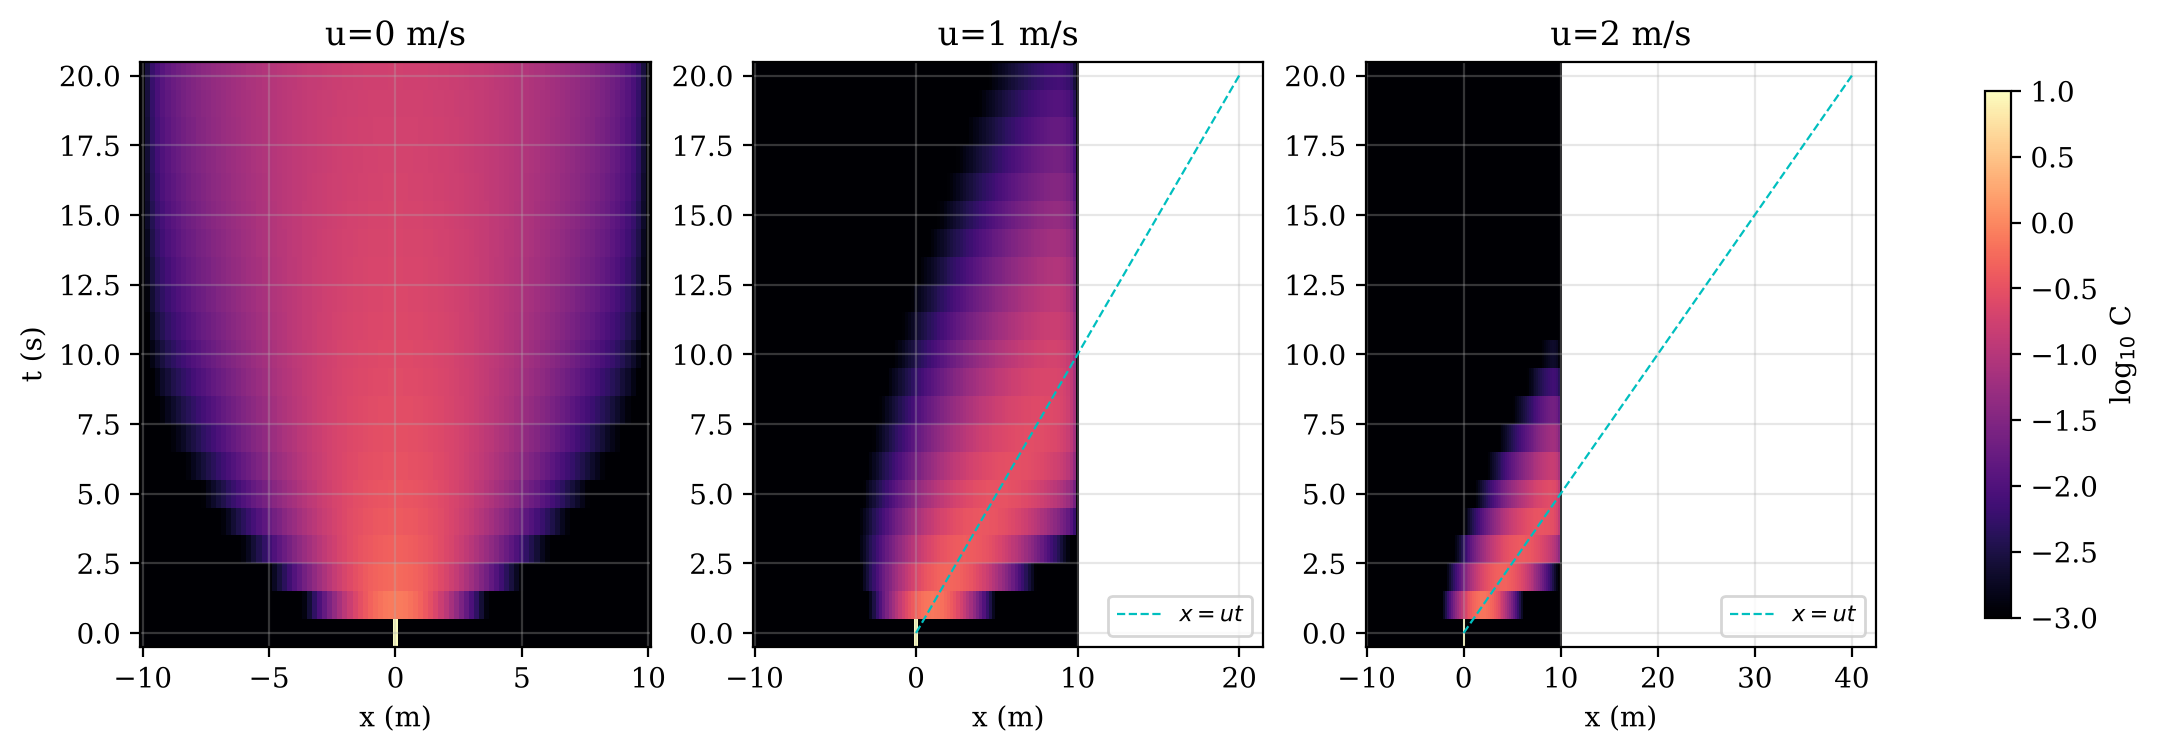
\includegraphics[width=\textwidth]{../results/fig3_space_time.png}
\caption{Space--time maps of $\log_{10}C$; the dashed line is the advective path $x=ut$.}\end{figure}

\subsection{Moment analysis}\label{sec:moments}
Mass $m_0=\int C\,dx$, centroid $\bar x$ and variance $\sigma^2$ were computed from every stored profile. Linear fits over the times when the plume is fully inside the domain give:
\begin{figure}[H]\centering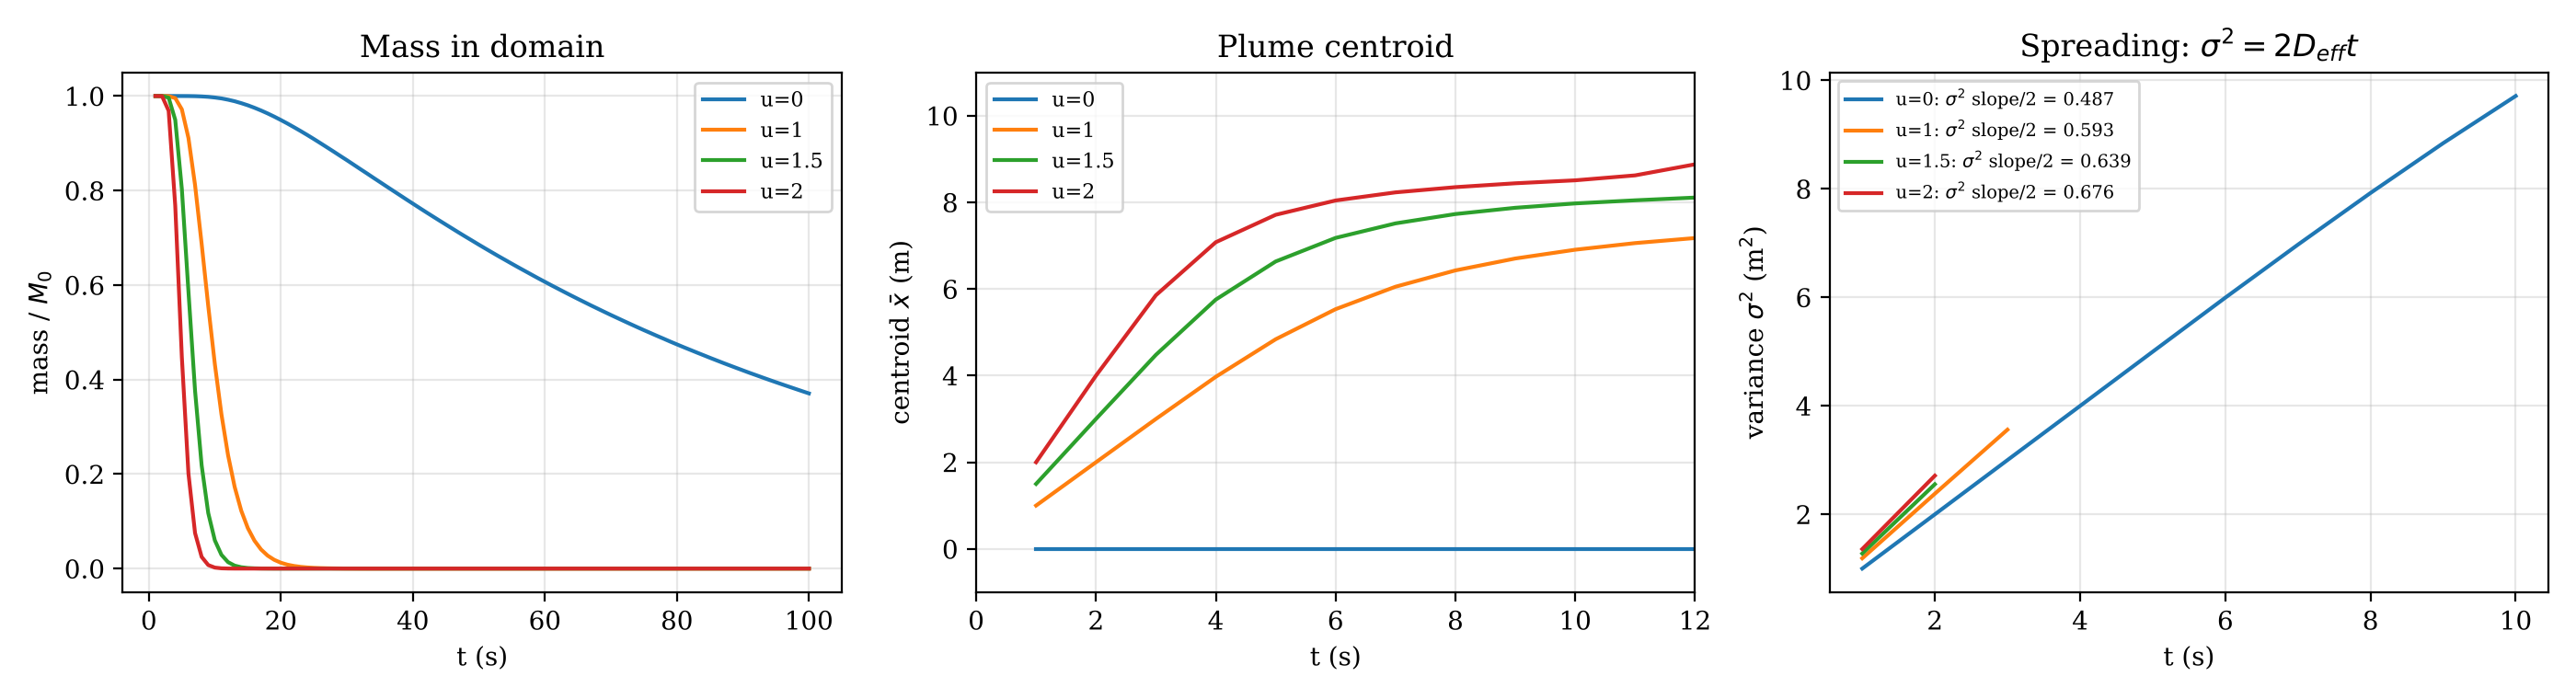
\includegraphics[width=\textwidth]{../results/fig2_moments.png}
\caption{Mass remaining in the domain, centroid and variance.}\end{figure}
\begin{table}[H]\centering\small
\begin{tabular}{ccccccc}\toprule
$u$ & $D_{num}$ (theory) & $D_{eff}$ (theory) & $D_{eff}$ from $\tfrac12 d\sigma^2/dt$ & Error & $d\bar x/dt$ & Fit points\\\midrule
0 & 0 & 0.500 & 0.487 & $-2.5\%$ & 0.000 & 10\\
1.0 & 0.095 & 0.595 & 0.593 & $-0.4\%$ & 0.999 & 3\\
1.5 & 0.139 & 0.639 & 0.639 & $0.0\%$ & 1.500 & 2\\
2.0 & 0.180 & 0.680 & 0.676 & $-0.5\%$ & 1.999 & 2\\\bottomrule
\end{tabular}\caption{Effective diffusivity and transport speed (m$^2$s$^{-1}$, m\,s$^{-1}$).}\end{table}
The measured spreading rates confirm the modified-equation prediction to within 0.5\% for the advected cases; the small deficit at $u=0$ comes from the slight loss of mass through the boundaries at $t\ge9$~s ($m_0=0.997M$ at 10~s). The centroid speed equals $u$, i.e.\ the scheme has no phase error in the mean transport, and mass is conserved exactly until the plume reaches a boundary.

\subsection{Original versus corrected code}
\begin{figure}[H]\centering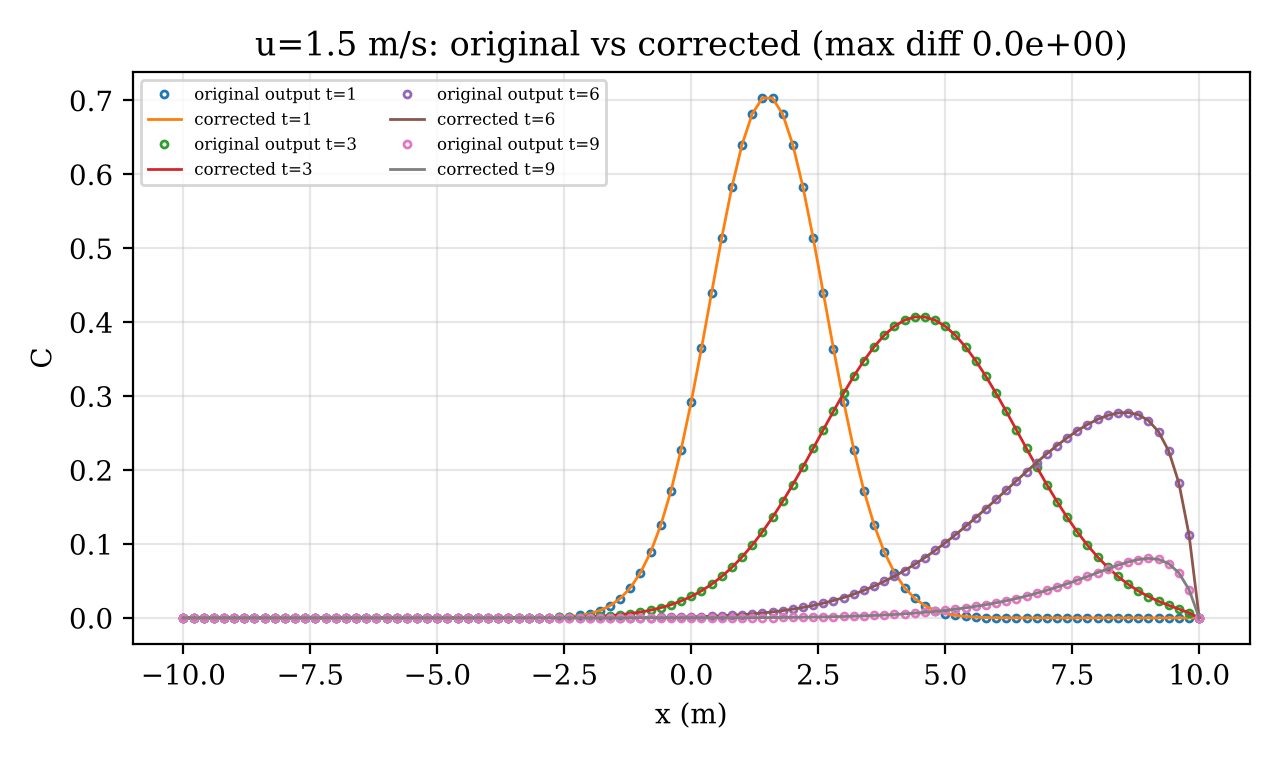
\includegraphics[width=0.66\textwidth]{../results/fig4_original_vs_corrected.png}
\caption{Original \texttt{results.txt} ($u=1.5$) and the corrected code: identical.}\label{fig:orig}\end{figure}

\section{Discussion: how to reduce the numerical diffusion}
Since $D_{num}\propto u\Delta x$, the error can be reduced by (i) refining the grid, which costs $\Delta t\propto\Delta x^2$ through the diffusion limit; (ii) using a second-order advection scheme (central or Lax--Wendroff, stable here because $\mathrm{Pe}_\Delta<2$), or (iii) a flux-limited TVD scheme that keeps monotonicity. With central advection the leading error becomes dispersive ($\mathcal{O}(\Delta x^2)C_{xxx}$) rather than diffusive.

\section{Conclusions}
\begin{itemize}
\item After two syntax corrections, the code reproduces the original results exactly and solves the advection--diffusion problem stably ($\mathrm{CFL}+2d\le0.35$) and monotonically.
\item The plume is advected at the correct speed and conserves mass, but first-order upwinding adds an artificial diffusivity $D_{num}=\tfrac12u\Delta x(1-\mathrm{CFL})$, i.e.\ 19--36\% of $D$ for $u=1$--2~m\,s$^{-1}$. This explains why the original plots show lower peaks at higher velocity than physical diffusion alone would give.
\item The modified-equation prediction is confirmed quantitatively by the second moment of the computed plumes (within 0.5\%).
\end{itemize}

\section*{Reproducing the results}
\texttt{bash run.sh} compiles \texttt{code/advection\_diffusion.c} for each velocity (only the \texttt{U} constant is substituted), runs it and calls \texttt{code/postprocess.py}.

\appendix\section{Source code (corrected)}
\lstinputlisting[language=C]{../code/advection_diffusion.c}
\end{document}
